% TEMPLATE.TEX
%
% Time-stamp: <2013-03-26 11:09 olenz>
%
% This is an extensively documented LaTeX file that shows how to
% produce a good-looking document with current LaTeX (11/2012).
%
% IMPORTANT!
%
%   Some obsolete commands and packages
% ----------|-------------------------------
% obsolete  |     Replacement in LATEX 2ε
% ----------|-------------------------------
%           | local            global/switch
% ----------|-------------------------------
% {\bf ...} | \textbf{...}     \bfseries
%     -     | \emph{...}       \em
% {\it ...} | \textit{...}     \itshape
%     -     | \textmd{...}     \mdseries
% {\rm ...} | \textrm{...}     \rmfamily
% {\sc ...} | \textsc{...}     \scshape
% {\sf ...} | \textsf{...}     \sffamily
% {\sl ...} | \textsl{...}     \slshape
% {\tt ...} | \texttt{...}     \ttfamily
%     -     | \textup{...}     \upshape
%
% DON'T USE \\ TO MAKE LINEBREAKS, INSTEAD JUST LEAVE A BLANK LINE!
%
\RequirePackage[l2tabu,orthodox]{nag} % turn on warnings because of bad style
\documentclass[a4paper,10pt,bibtotoc]{scrartcl}
%
\usepackage[bottom=3.5cm, top=3cm]{geometry}
\usepackage{subcaption}
\captionsetup[subfigure]{list=true, position=top}
\usepackage{float}
%%%%%%%%%%%%%%%%%%%%%%%%%%%%%%%%%%%%
% KOMA CLASSES
%%%%%%%%%%%%%%%%%%%%%%%%%%%%%%%%%%%%
%
% The class "scrartcl" is one of the so-called KOMA-classes, a set of
% very well done LaTeX-classes that produce a very European layout
% (e.g. titles with a sans-serif font).
%
% The KOMA classes have extensive documentation that you can access
% via the commands:
%   texdoc scrguide # in German
%   texdoc scrguien # in English
%
%
% The available classes are:
%
% scrartcl - for "articles", typically for up to ~20 pages, the
%            highest level sectioning command is \section
%
% scrreprt - for "reports", typically for up to ~200 pages, the
%            highest level sectioning command is \chapter
%
% scrbook  - for "books", for more than 200 pages, the highest level
%            sectioning command is \part.
%
% USEFUL OPTIONS
%
% a4paper  - Use a4 paper instead of the default american letter
%            format.
%
% 11pt, 12pt, 10pt
%          - Use a font with the given size.
%
% bibtotoc - Add the bibliography to the table of contents
%
% The KOMA-script classes have plenty of options to modify

% This allows to type UTF-8 characters like ä,ö,ü,ß
\usepackage[utf8]{inputenc}

\usepackage[T1]{fontenc}        % Tries to use Postscript Type 1 Fonts for better rendering
\usepackage{lmodern}            % Provides the Latin Modern Font which offers more glyphs than the default Computer Modern
\usepackage[intlimits]{amsmath} % Provides all mathematical commands
\usepackage{amssymb}
\usepackage{hyperref}           % Provides clickable links in the PDF-document for \ref
\usepackage{graphicx}            % Allow you to include images (like graphicx). Usage: \includegraphics{path/to/file}

% Allows to set units
\usepackage[ugly]{units}        % Allows you to type units with correct spacing and font style. Usage: $\unit[100]{m}$ or $\unitfrac[100]{m}{s}$

% Additional packages
\usepackage{url}                % Lets you typeset urls. Usage: \url{http://...}
\usepackage{breakurl}           % Enables linebreaks for urls
\usepackage{xspace}             % Use \xpsace in macros to automatically insert space based on context. Usage: \newcommand{\es}{ESPResSo\xspace}
\usepackage{xcolor}             % Obviously colors. Usage: \color{red} Red text
\usepackage{booktabs}           % Nice rules for tables. Usage \begin{tabular}\toprule ... \midrule ... \bottomrule
\usepackage{siunitx}


% Source code listings
\usepackage{listings}           % Source Code Listings. Usage: \begin{lstlisting}...\end{lstlisting}
\lstloadlanguages{python}
\definecolor{lightpurple}{rgb}{0.8,0.8,1}

\lstset{
stepnumber=1,
numbersep=5pt,
numberstyle=\small\color{black},
basicstyle=\ttfamily,
%keywordstyle=\color{black},
%commentstyle=\color{black},
%stringstyle=\color{black},
frame=single,
tabsize=4,
language = python,
backgroundcolor=\color{black!5}}

\usepackage{float}

\begin{document}

\titlehead{Simulation Methods in Physics I \hfill WS 2019/2010}
\title{Report for Worksheet 5: Monte Carlo}
\author{Markus Baur and David Beyer}
\date{\today}
\maketitle

\tableofcontents
\section{Simple Sampling -- Integration}
The Python code for the following section can be found in the file ex\_5\_2.py.
\subsection{Exact Integration}
A plot of the function $f(x)$ on the interval $\left[0.1,50.0\right]$ is shown in \autoref{fig:fig1}. 
We can see that the function is almost zero for most values of $x$, disrupted by sharp peaks.
This means that we will need a lot of samples to obtain an acceptable value using simple sampling.
The situation is thus in a way similiar to the problem of equilibrium statistical mechanics, where the Boltzmann factor is extremly small for most points of the phase space and simple sampling is not an efficient method.
\begin{figure}
	\centering
	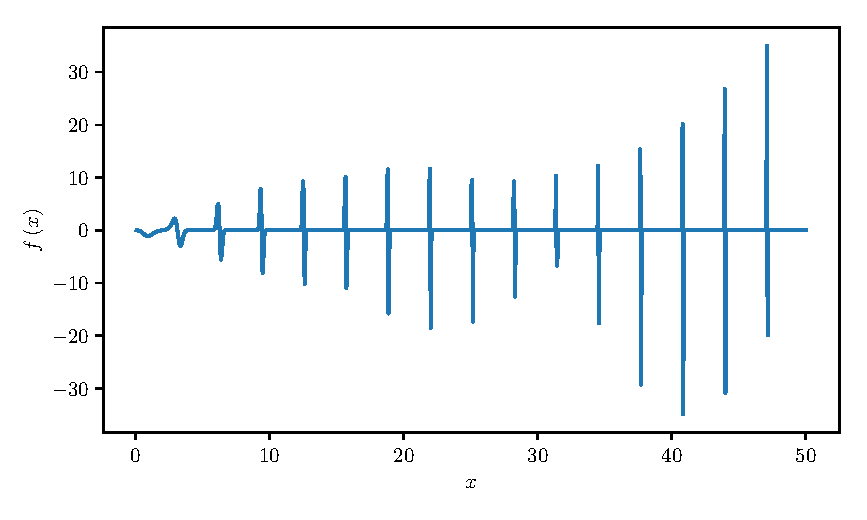
\includegraphics[width=\linewidth]{plotf.pdf}
	\caption{Plot of the function $f(x)$ on the interval $\left[0.1,50.0\right]$.}
	\label{fig:fig1}
\end{figure}

To obtain the exact integral of $f(x)$ over an interval $\left[a, b\right]$, we wrote the function exact\_integral, which uses the SymPy module to calculate a closed expression of the integral:
\begin{lstlisting}
def exact_integral(a, b):
    x = Symbol('x')
    ret = integrate((-2 * x**2 * sin(x) * cos(x) - 2 * x * sin(x)**2)\
        * exp(-x**2 * sin(x)**2), (x, a, b))
    return ret
\end{lstlisting}
The obtained value is
\begin{align}
\int_{0.1}^{50.0}\mathrm{d}x\,f(x)\approx -0.9999.
\end{align}
(Note that the approximate sign $\approx$ only appears because we give the result as a number instead of in terms of exponential functions.)

\subsection{Monte Carlo Integration}
To perform a Monte Carlo integration using simple sampling, we wrote the following function:
\begin{lstlisting}
def simple_sampling(f, a, b, N):
    dx = (b - a) / N
    ret = 0.0
    sample = 0.0
    squared_sum  = 0.0
    for i in range(N):
        sample = f((b - a) * np.random.random_sample() + a)
        ret += sample
        squared_sum += sample ** 2
    error = np.sqrt(squared_sum - (ret ** 2) / N)
    error *= (b - a) / np.sqrt(N * (N-1))
    ret *= dx
    return ret, error
\end{lstlisting}
The has as its arguments the function $f$ which has to be integrated, the limits $a$ and $b$ of the interval and the number of samples $N$. 
Furthermore, the function also calculates the an estimate for the error of the calculated value.

To compute an estimate of the error for the obtained integral, we note that the $N$ different samples $f(x_i)$ are uncorrelated in the case of simple sampling.
The unbiased estimator of the variance of $f$ is given by
\begin{align}
\hat{\sigma}(f)^2 = \frac{1}{N-1}\left(\sum_{i=1}^{N}f(x_i)^2-\frac{1}{N}\left(\sum_{i=1}^{N}f(x_i)\right)^2\right).
\end{align}
Because the samples are uncorrelated and statistically independent, we can calculate the unbiased estimator of the variance of the integral $I$ as
\begin{align}
\hat{\sigma}(I)^2 &= \frac{\left(a-b\right)^2}{N^2}\sum_{i=1}^{N} \hat{\sigma}(f)^2 = \frac{\left(a-b\right)^2\hat{\sigma}(f)^2}{N}\\
&=\frac{\left(a-b\right)^2}{N\left(N-1\right)}\left(\sum_{i=1}^{N}f(x_i)^2-\frac{1}{N}\left(\sum_{i=1}^{N}f(x_i)\right)^2\right)
\end{align}
which leads to an estimation of the error of $I$ that is given by
\begin{align}
\epsilon(I)=\sqrt{\frac{\left(a-b\right)^2}{N\left(N-1\right)}\left(\sum_{i=1}^{N}f(x_i)^2-\frac{1}{N}\left(\sum_{i=1}^{N}f(x_i)\right)^2\right)}.
\end{align}
This error estimation is equal to the estimator for the standard error of the mean of $f$ times the length of the interval $[a,b]$, which is not surprising considering that $I$ is given by $\left(b-a\right)\cdot \overline{f}$.

\autoref{fig:fig2} shows a plot of the Monte Carlo estimate of the integral as function of the number of samples. 
We can see that the value fluctuates wildly for small sample numbers $N$, but these fluctuations become smaller as $N$ becomes larger and the Monte Carlo estimate converges towards the real value of the integral.

\autoref{fig:fig3} shows a plot of the statistical and actual errors of the Monte Carlo estimate of the integral as function of the number of samples. 
Both of these errors become smaller as $N$ increases.

\begin{figure}
	\centering
	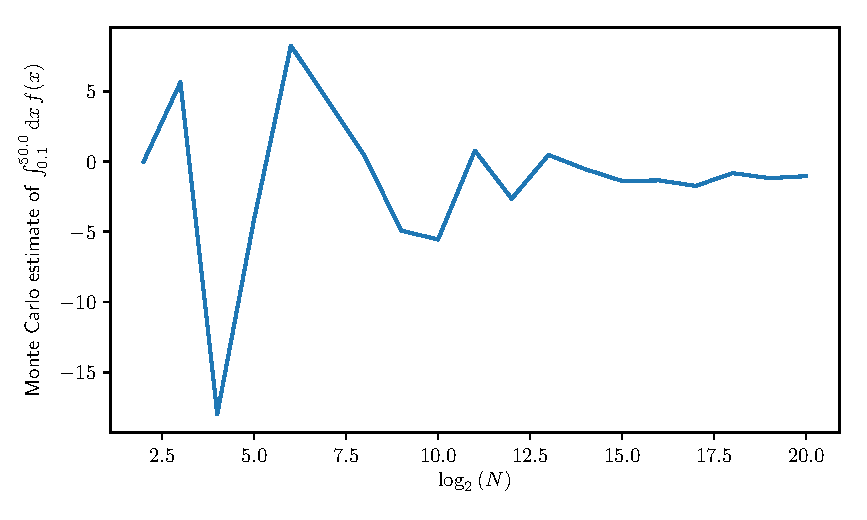
\includegraphics[width=\linewidth]{integral_f.pdf}
	\caption{Plot of the Monte Carlo estimate of the integral $\int_{0.1}^{50.0}\mathrm{d}x\,f(x)$ as function of the number of samples $N$ (logarithmic representation).}
	\label{fig:fig2}
\end{figure}

\begin{figure}
	\centering
	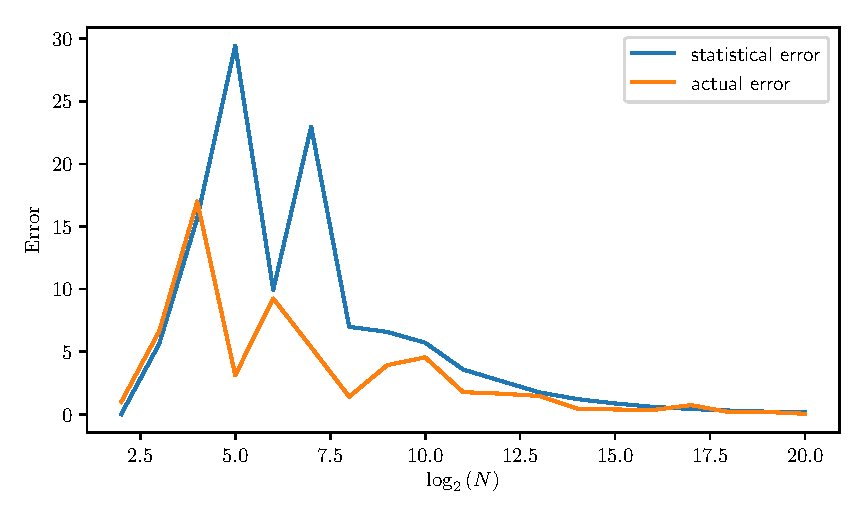
\includegraphics[width=\linewidth]{error_integral.pdf}
	\caption{Plot of the statistical and actual error of the Monte Carlo estimate of the integral $\int_{0.1}^{50.0}\mathrm{d}x\,f(x)$ as function of the number of samples $N$ (logarithmic representation).}
	\label{fig:fig3}
\end{figure}

\newpage
\section{Importance Sampling -- Metropolis-Hastings Algorithm}
The Python code for the following section can be found in the file ex\_5\_3.py.
\subsection{Metropolis-Hastings-Algorithm}
We implemented the function metropolis in the following way:
\begin{lstlisting}
def metropolis(N, P, trial_move, phi0, dx):
    ret = []
    ret.append(phi0)
    phi = phi0
    phi_next = phi0
    counter = 0
    for i in range(N):
        #Perform trial move
        phi_next = trial_move(phi, dx)
        
        #Generate a random number
        r = np.random.random_sample()
        
        #Decide if new state is accepted
        if r < min(1, P(phi_next)/P(phi)):
            phi = phi_next
            counter += 1
        
        #Add new state to the list
        ret.append(phi)
    #Calculate the acceptance rate
    acceptance_rate = counter / N
    return ret, acceptance_rate
\end{lstlisting}
The function metropolis has as its arguments the number of steps N, the probability distribution P which is sampled, the function trial\_move which generatesa new state from the present state. 
$dx$ describes the maximum size of a single step.
The sampling is performed in the following way: first, a new state phi\_next is proposed using the function trial\_move.
Next, a random number $r\in[0,1)$ is generated using numpy.random.
This random number is then used to decide if the proposed state is accepted or not, if it is accepted, phi is assigned the new state and the (acceptance) counter is increased by 1.
Last, the new state is appended to the list of states.
The procedure just described is repeated N times, at the end, the acceptance rate is calculated by dividing the counter by the total number of steps N.
Finally, the list of states and the acceptance rate are returned.

\subsection{Sampling a Gaussian Distribution}
We now use the function metropolis which was described above to sample number from the Gaussian distribution
\begin{align}
p(x) = \frac{\exp\left(-x^2\right)}{\sqrt{2}}.
\end{align}
For the trial move, we randomly select a number in the interval $\left[-dx, dx\right]$ according to a uniform probability distribution:
\begin{lstlisting}
def trial_move(x, dx):
    r = 2 * dx * np.random.random_sample() - dx
    ret = x + r
    return ret
\end{lstlisting}
\autoref{fig:fig4} -- \autoref{fig:fig7} compare the sampled Gaussian distribution $p(x)$ with the normalized histograms which were obtained by sampling $p(x)$ 400000 times using the Metropolis-Hastings-algorithm for different maximum step sizes $dx$.
The measured acceptance rates for the different step sizes were
\begin{table}[H]
\center
\begin{tabular}{cc}
\toprule
$dx$ & acceptance rate\\\midrule
0.1 & 0.97147\\
1.0 & 0.7292125\\
10.0 & 0.1137475\\
100.0 & 0.0113825\\
\bottomrule
\end{tabular}
\end{table}
\noindent As we would expect, the acceptance rate decreases as $dx$ increases because the Gaussian distribution rapidly falls off to zero.
The histogram which approximates the Gaussian distribution the best was obtained for $dx=1.0$ which corresponds to an acceptance rate of $0.7292125$.
The quality of the results for the Metropolis-Hastings-algorithm is determined by two competing effects: on the one hand, the step size should not be too small, because in this case we need a huge number of steps to sample all relevant points.
On the other hand, the step size should not be too large, because then the acceptance rate will be small and we will also need a large number of samples to obtain accurate results.

\begin{figure}[H]
	\centering
	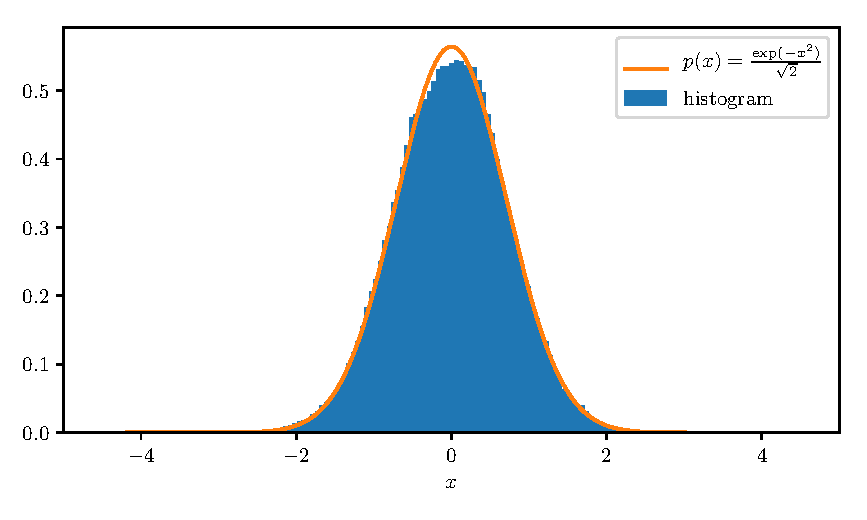
\includegraphics[width=\linewidth]{hist01.pdf}
	\caption{Comparison of the sampled Gaussian distribution $p(x)$ and the normalized histogram for a maximum step size of $dx=0.1$ and 400000 samples.}
	\label{fig:fig4}
	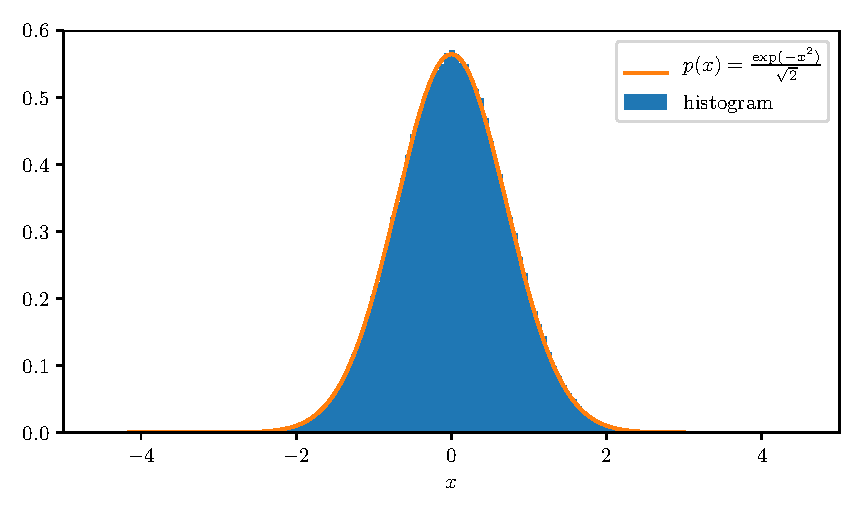
\includegraphics[width=\linewidth]{hist1.pdf}
	\caption{Comparison of the sampled Gaussian distribution $p(x)$ and the normalized histogram for a maximum step size of $dx=1.0$ and 400000 samples.}
	\label{fig:fig5}
\end{figure}

\begin{figure}[H]
	\centering
	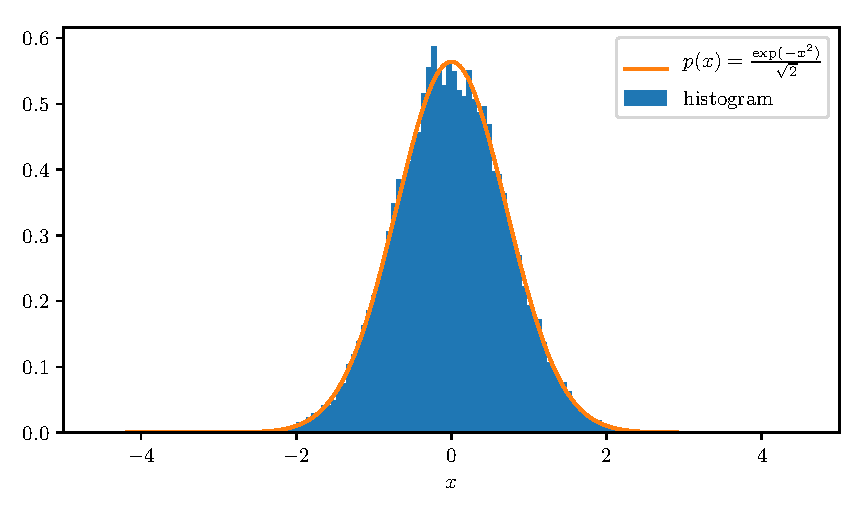
\includegraphics[width=\linewidth]{hist10.pdf}
	\caption{Comparison of the sampled Gaussian distribution $p(x)$ and the normalized histogram for a maximum step size of $dx=10.0$ and 400000 samples.}
	\label{fig:fig6}
	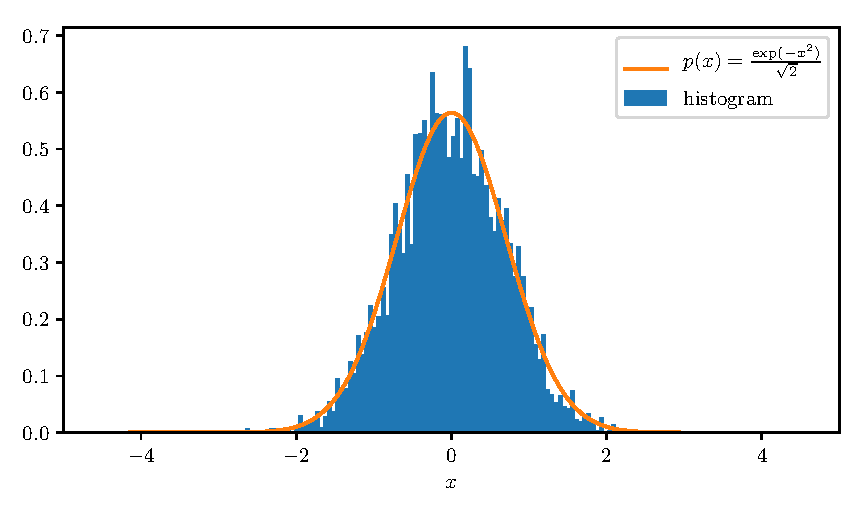
\includegraphics[width=\linewidth]{hist100.pdf}
	\caption{Comparison of the sampled Gaussian distribution $p(x)$ and the normalized histogram for a maximum step size of $dx=100.0$ and 400000 samples.}
	\label{fig:fig7}
\end{figure}


\section{Simulate the Ising Model}
The Python code for the following section can be found in the file ex\_5\_4.py.
\subsection{Exact Summation}
To perform an exact summation of the Ising model, we implemented three functions. 
The function ising\_mean returns the mean value of the energy and of the absolute value of the magnetization for the Ising model with $Nx\cdot Ny$ spins at a given temperature $T$:
\begin{lstlisting}
def ising_mean(Nx, Ny, T):
    Z = 0.0
    mean_energy = 0.0
    mean_magnetization = 0.0
    iterator = itertools.product([-1, +1], repeat = Nx*Ny)
    for i in iterator:
        m = calculate_magnetization(list(i))
        E = calculate_energy(list(i), Nx, Ny)
        boltzmann = np.exp( -E / T)
        Z += boltzmann
        mean_energy += E * boltzmann
        mean_magnetization +=\
        np.abs(calculate_magnetization(list(i))) * boltzmann
    mean_energy /= (Z * Nx * Ny)
    mean_magnetization /= (Z * Nx * Ny)
    return mean_energy, mean_magnetization
\end{lstlisting}
To describe a specific spin configuration, we use a list of length $Nx\cdot Ny$ with entries $+1$ or $-1$ corresponding to the value of a given spin.
In order to loop over all possible configurations of the spin system, we use the iterator
\begin{lstlisting}
iterator = itertools.product([-1, +1], repeat = Nx*Ny).
\end{lstlisting}
For each configuration, we calculate the energy and the magnetization using the functions calculate\_energy calculate\_magnetization (defined below).
We then calculate the Boltzmann factor for this energy and add it to $Z$ (which will become the partition function).
Furthermore, we add the weighted values of the energy and the absolute value of the magnetization to mean\_energy and mean\_magnetization.
After the loop over all configurations has been performed, the mean energy and magnetization are normalized to obtain the mean energy and magnetization of a single spin and returned.

The function which returns the energy has the following form, it calculates the energy defined by the next neighbour interaction of the Ising model (we set the coupling constant $J$, the magnetic moment of one spin $m$ and the Boltzmann constant equal to 1):
\begin{lstlisting}
def calculate_energy(spin_config, Nx, Ny):
    ret = 0.0
    for nx in range(Nx):
        for ny in range(Ny):
            ret += -0.5 * spin_config[nx * Ny + ny]\
            * (spin_config[((nx - 1) % Nx) * Ny + ny]\
                + spin_config[((nx + 1) % Nx) * Ny + ny]\
                + spin_config[nx * Ny + (ny - 1) % Ny]\
                + spin_config[nx * Ny + (ny + 1) % Ny])
    return ret
\end{lstlisting}
To calculate the magnetization of a given configuration, we simply sum over the values of all spins:
\begin{lstlisting}
def calculate_magnetization(spin_config):
    return np.sum(spin_config)
\end{lstlisting}

\begin{figure}[H]
	\centering
	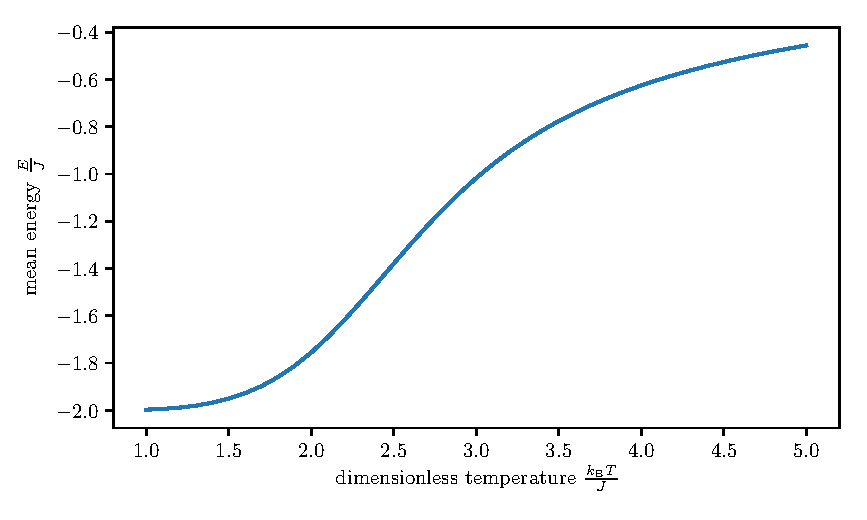
\includegraphics[width=\linewidth]{energy_exact.pdf}
	\caption{Plot of the mean energy per spin obtained by exact summation of the Ising model with periodic boundary conditions on a grid with $4\times 4$ spins as a function of temperature.}
	\label{fig:fig8}
	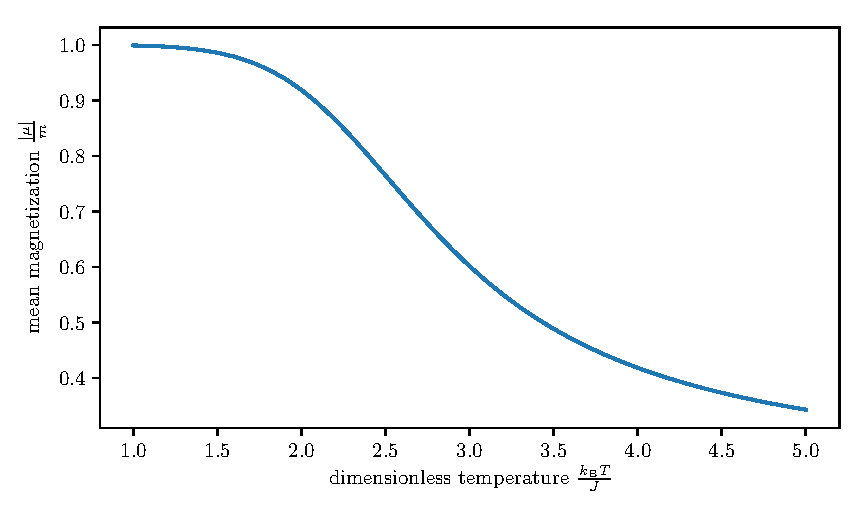
\includegraphics[width=\linewidth]{magnetization_exact.pdf}
	\caption{Plot of the mean magnetization per spin obtained by exact summation of the Ising model with periodic boundary conditions on a grid with $4\times 4$ spins as a function of temperature.}
	\label{fig:fig9}
\end{figure}

\noindent\autoref{fig:fig8} and \autoref{fig:fig9} show the mean energy and magnetization per spin as a function of temperature.
As we would expect, the mean energy rises as the temperature is increased, this can be explained by the fact that the Boltzmann factor $\exp\left(-E/k_\mathrm{B}T\right)$ becomes larger for a given energy as $T$ increases, making higher energies more probable. 
The mean magnetization on the other hand decreases as the temperature rises, this behaviour can also be understood qualitatively:
In general, configurations where many spins are parallel have a lower energy than states with less order, they also have a high magnetization. 
Since many parallel spins correspond to a lower energy, the statistical weight of these states decreases as the temperature is increased which leads to a lowering of the mean magnetization.
Effectively, a higher temperature leads to a weaker coupling between neighbouring spins, because in the Boltzmann factor, only the ratio $J/k_\mathrm{B}T$ appears.

\subsection{Monte-Carlo Simulation}
To perform a Monte-Carlo simulation of the Ising model, we implemented the function ising\_monte\_carlo:
\begin{lstlisting}
def ising_monte_carlo(N_MC_STEPS, Nx, Ny, T):
    N_SPINS = Nx * Ny
    spin_config = [(-1) ** np.random.randint(0, high=2)\
    for i in range(N_SPINS)]
    energy = calculate_energy(spin_config, Nx, Ny)
    magnetization = calculate_magnetization(spin_config)
    mean_energy = 0.0
    mean_magnetization = 0.0
    
    for i in range(N_MC_STEPS):
        #Choose a random spin to flip
        random_spin = np.random.randint(0, high=N_SPINS)
        
        #Calculate the coordinates of the spin
        ny = random_spin % Ny
        nx = int((random_spin - ny) / Ny)
        
        #Calculate the new energy for this configuration
        energy_trial = energy + 2 * spin_config[nx * Ny + ny]\
                * (spin_config[((nx - 1) % Nx) * Ny + ny]\
                + spin_config[((nx + 1) % Nx) * Ny + ny]\
                + spin_config[nx * Ny + (ny - 1) % Ny]\
                + spin_config[nx * Ny + (ny + 1) % Ny])
        
        #Decide if new spin configuration is accepted
        if np.random.random_sample() <\
        min(1, np.exp( (energy - energy_trial)/ T)):
            spin_config[random_spin] *= -1
            energy = energy_trial
            magnetization += 2 * spin_config[random_spin]
        
        mean_energy += energy
        mean_magnetization += np.abs(magnetization)
        
    mean_energy /= (N_MC_STEPS * N_SPINS)
    mean_magnetization /= (N_MC_STEPS * N_SPINS)
    return mean_energy, mean_magnetization
\end{lstlisting}
The arguments of the function are the number of Monte-Carlo steps N\_MC\_STEPS, the number of spins in the $x$- and $y$-direction Nx and Ny and the dimensionless temperature T.
As before, we store a spin configuration as a list of length Nx$\cdot$Ny.
To initialize the system, we produce a random intial condition using 
\begin{lstlisting}
spin_config = [(-1) ** np.random.randint(0, high=2)\
for i in range(N_SPINS)]
\end{lstlisting}
The Monte-Carlo sampling is performed N\_MC\_STEPS times using a for loop, it is done in this way: 
First, we choose a random spin to flip by drawing a random number from a uniform distribution over the integers in the interval $[0,\mathrm{N\_SPINS})$, this random number is used as the index in the list of spins to determine the random spin $\sigma_{i,j}$.
Next, the energy of the new configuration is calculated by subtracting
\begin{align}
-2\cdot 2\cdot \frac{1}{2}\sigma_{i,j,\mathrm{old}}\left(\sigma_{i-1, j}+\sigma_{i+1, j}+\sigma_{i, j-1}+\sigma_{i, j+1}\right) = 2\cdot 2\cdot E_{i,j,\mathrm{old}}
\end{align}
from the current energy.
The term we subtract can be explained in the following way: 
We subtract 4 times the energy of the chosen spin in the old configuration. 
The energy is subtracted because changing the sign of the spin will also change the sign of the energy. 
One factor of two appears because the interaction energy is symmetric, so we have to take into account the interaction energy of the chosen spin with its neighbours but also the other way around. 
The other factor of two appears because we first have to compensate for the energy in the old configuration and then add the interaction energy of the spin with its neighbours.
Once we have calculated the energy of the proposed new state, we draw a random number from a uniform distribution over $[0,1)$ and decide if the new state is accepted by comparing it with the Boltzmann factor for the energy difference.
If the new configuration is accepted, we update the spin confugration, energy and magnetization.
We then add the energy and magnetization to mean\_energy and mean\_magnetization.
Once we have performed N\_MC\_STEPS, the mean energy and magnetization are normalized and returned.

\autoref{fig:fig10} and \autoref{fig:fig11} compare the results of the exact summation (which were presented above) to the results of a Monte Carlo simulation with 10000 samples. 
We observe that the values obtained from the Monte Carlo simulation fluctuate around the exact results.
\autoref{fig:fig12} and \autoref{fig:fig13} compare the results of the exact summation to the results of a Monte Carlo simulation with 1000000 samples (100 times as many as before), compared to the Monte Carlo simulation above, the deviation from the exact solution is much smaller. 

\begin{figure}[H]
	\centering
	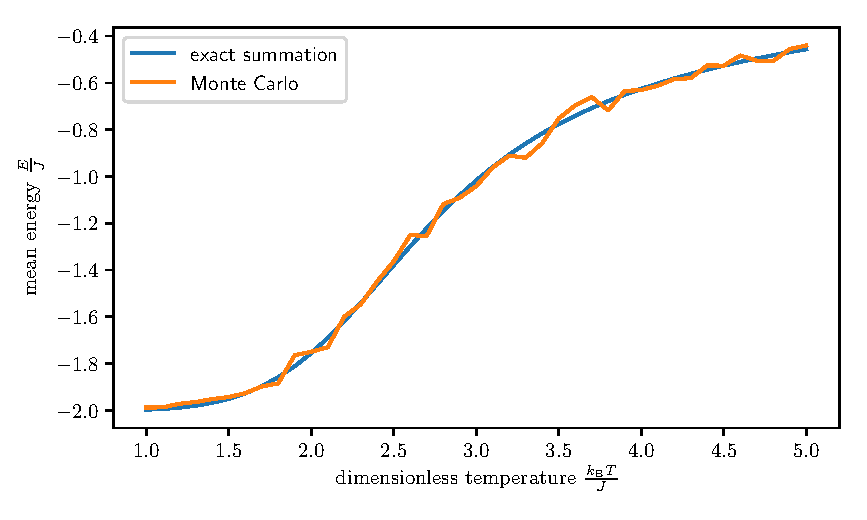
\includegraphics[width=\linewidth]{energy_mc.pdf}
	\caption{Plot of the mean energy per spin obtained by exact summation and Monte Carlo simulation (10000 samples) of the Ising model with periodic boundary conditions on a grid with $4\times 4$ spins as a function of temperature.}
	\label{fig:fig10}
	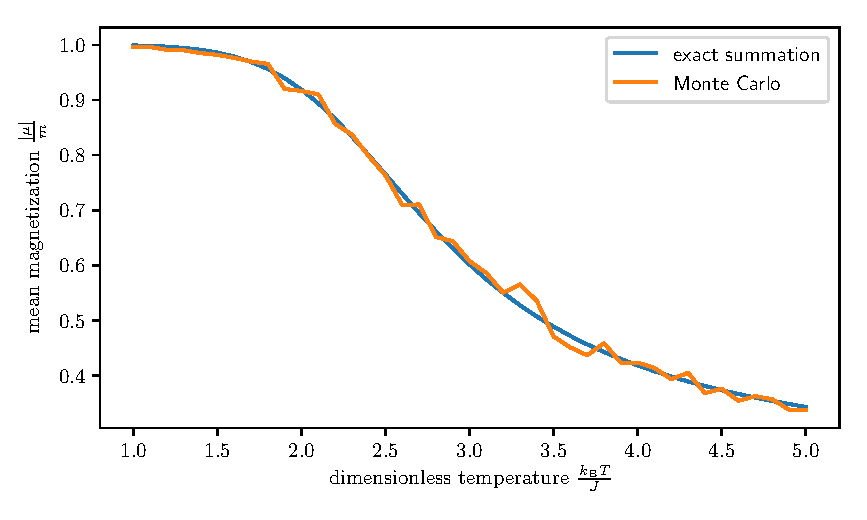
\includegraphics[width=\linewidth]{magnetization_mc.pdf}
	\caption{Plot of the mean energy per spin obtained by exact summation and Monte Carlo simulation (10000 samples) of the Ising model with periodic boundary conditions on a grid with $4\times 4$ spins as a function of temperature.}
	\label{fig:fig11}
\end{figure}

\begin{figure}[H]
	\centering
	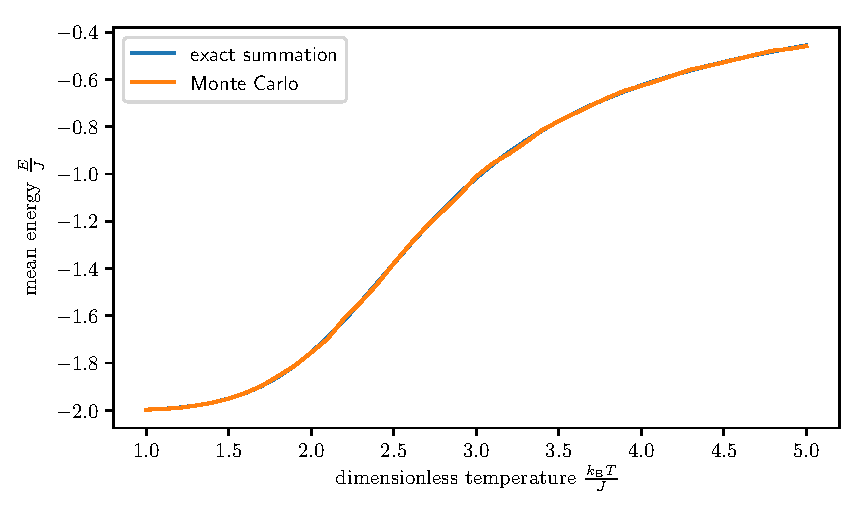
\includegraphics[width=\linewidth]{energy_mc_moresamples.pdf}
	\caption{Plot of the mean energy per spin obtained by exact summation and Monte Carlo simulation (1000000 samples) of the Ising model with periodic boundary conditions on a grid with $4\times 4$ spins as a function of temperature.}
	\label{fig:fig12}
	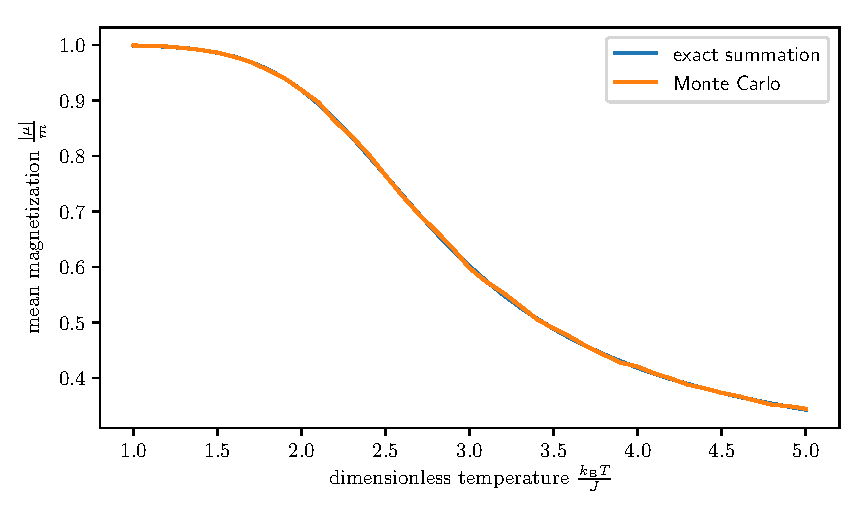
\includegraphics[width=\linewidth]{magnetization_mc_moresamples.pdf}
	\caption{Plot of the mean energy per spin obtained by exact summation and Monte Carlo simulation (1000000 samples) of the Ising model with periodic boundary conditions on a grid with $4\times 4$ spins as a function of temperature.}
	\label{fig:fig13}
\end{figure}

\end{document}
